\hypertarget{test__replace_8cpp}{}\subsection{test\+\_\+replace.\+cpp File Reference}
\label{test__replace_8cpp}\index{test\+\_\+replace.\+cpp@{test\+\_\+replace.\+cpp}}


An example of doing regex replace with J\+P\+C\+R\+E2.  


{\ttfamily \#include $<$iostream$>$}\\*
{\ttfamily \#include \char`\"{}jpcre2.\+hpp\char`\"{}}\\*
Include dependency graph for test\+\_\+replace.\+cpp\+:\nopagebreak
\begin{figure}[H]
\begin{center}
\leavevmode
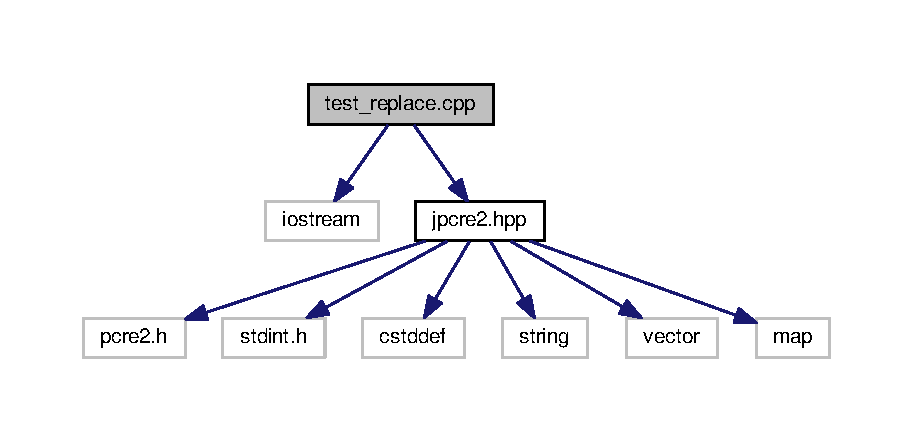
\includegraphics[width=350pt]{test__replace_8cpp__incl}
\end{center}
\end{figure}


\subsubsection{Detailed Description}
An example of doing regex replace with J\+P\+C\+R\+E2. 


\begin{DoxyCodeInclude}
\textcolor{comment}{/**@file test\_replace.cpp}
\textcolor{comment}{ * An example of doing regex replace with JPCRE2}
\textcolor{comment}{ * @include test\_replace.cpp}
\textcolor{comment}{ * @author [Md Jahidul Hamid](https://github.com/neurobin)}
\textcolor{comment}{ * */}

\textcolor{preprocessor}{#include <iostream>}
\textcolor{preprocessor}{#include "\hyperlink{jpcre2_8hpp}{jpcre2.hpp}"}


\textcolor{keywordtype}{int} main()\{
    \hyperlink{classjpcre2_1_1Regex}{jpcre2::Regex} re;     \textcolor{comment}{/// This is not supposed to throw any exception.}
\textcolor{comment}{}\textcolor{comment}{}
\textcolor{comment}{    ///Compile the pattern}
\textcolor{comment}{}    \textcolor{keywordflow}{try}\{re.\hyperlink{classjpcre2_1_1Regex_a85d9a514ea86ae68533223adac6c6bd8}{setPattern}(\textcolor{stringliteral}{"(?:(?<word>[?.#@:]+)|(?<word>\(\backslash\)\(\backslash\)w+))\(\backslash\)\(\backslash\)s*(?<digit>\(\backslash\)\(\backslash\)d+)"})     \textcolor{comment}{//Set various
       parameters}
          .\hyperlink{classjpcre2_1_1Regex_ab1af1471339602446d8221b8c97c6b55}{addModifier}(\textcolor{stringliteral}{"&Jin"})                                                     \textcolor{comment}{//modifier &
       == jpcre2::VALIDATE\_MODIFIER}
          .\hyperlink{classjpcre2_1_1Regex_a2c7dcf12f26b2b046e147b013c8b5087}{addPcre2Option}(0)                                                       \textcolor{comment}{//...}
          .\hyperlink{classjpcre2_1_1Regex_aad1d5ef1e87f762f68a587eec4022e69}{compile}();\}                                                             \textcolor{comment}{//Finally compile
       it.}
    \textcolor{keywordflow}{catch}(\hyperlink{classjpcre2_1_1Except}{jpcre2::Except}& e)\{std::cerr<<e.\hyperlink{classjpcre2_1_1Except_aa9f557fe16222ac89a30c438212c0c09}{getErrorMessage}();\}
        
    \textcolor{comment}{/******************************************************************************************************
      ************}
\textcolor{comment}{     * Use try catch block to catch any exception and avoid unexpected termination of the program in case
       of error}
\textcolor{comment}{     * All jpcre2 exceptions are of type jpcre2::Except}
\textcolor{comment}{     * ****************************************************************************************************
      ************/}
    
    \textcolor{comment}{//subject string}
    std::string s=\textcolor{stringliteral}{"I am a string with words and digits 45 and specials chars: ?.#@ 443 অ আ ক খ গ ঘ  56"};
    
    \textcolor{keywordflow}{try}\{std::cout<<\textcolor{stringliteral}{"\(\backslash\)nreplaced string: \(\backslash\)n"}<<
        re.\hyperlink{classjpcre2_1_1Regex_ae7235a991492fa88f1bd3fb02d59cd0a}{initReplace}()                                                    \textcolor{comment}{//Invoke the
       initReplace() function}
          .\hyperlink{classjpcre2_1_1RegexReplace_a46eefdb105827920bebc8436721fa4cb}{setSubject}(s)                                                    \textcolor{comment}{//Set various
       parameters}
          .\hyperlink{classjpcre2_1_1RegexReplace_af1069f489de9b343493da2dc77b04c73}{setReplaceWith}(\textcolor{stringliteral}{"(replaced:$1)(replaced:$2)(replaced:$\{word\})"})   \textcolor{comment}{//...}
          .\hyperlink{classjpcre2_1_1RegexReplace_a06a57430f62058822d48722a2a6425d7}{addModifier}(\textcolor{stringliteral}{"~xE"})                                               \textcolor{comment}{//modifier ~ ==
       jpcre2::ERROR\_ALL}
          .\hyperlink{classjpcre2_1_1RegexReplace_a3cfd03568b23bebcbb530a2c120b5d33}{addPcre2Option}(0)                                                \textcolor{comment}{//...}
          .\hyperlink{classjpcre2_1_1RegexReplace_afd087fa7a9bfedec802d1a3dd7edbdd0}{replace}();                                                       \textcolor{comment}{//Finally perform the
       replace operation.}
    \}
    \textcolor{keywordflow}{catch}(\hyperlink{classjpcre2_1_1Except}{jpcre2::Except}& e)\{std::cerr<<e.\hyperlink{classjpcre2_1_1Except_aa9f557fe16222ac89a30c438212c0c09}{getErrorMessage}();\}
    
    \textcolor{keywordflow}{return} 0;
\}
\end{DoxyCodeInclude}
 \begin{DoxyAuthor}{Author}
\href{https://github.com/neurobin}{\tt Md Jahidul Hamid} 
\end{DoxyAuthor}
